% Standalone supplementary PDF: same appendix content as main.tex's \appendix block, built as
% its own document for the separate supplementary upload ICLR accepts alongside the main PDF.
% Uses the same style-detection logic as main.tex -- see iclr2027_fallback_shim.sty for why a
% placeholder is used until the real iclr2027_conference.sty is available.
\documentclass{article}

\usepackage{iftex}
\newif\ifhasrealstyle
\IfFileExists{iclr2027_conference.sty}{\hasrealstyletrue}{\hasrealstylefalse}
\ifhasrealstyle
  \usepackage{iclr2027_conference}
\else
  \usepackage{iclr2027_fallback_shim}
\fi

\usepackage[utf8]{inputenc}
\usepackage[T1]{fontenc}
\usepackage{amsmath,amssymb,amsfonts}
\usepackage{graphicx}
\usepackage{booktabs}
\usepackage{multirow}
\usepackage{xcolor}
\usepackage{pifont}
% No TikZ/PGFPlots needed here: this document only \input's sections/appendix.tex, whose
% figure (the qualitative confusion-matrix/calibration panel) is a pre-rendered vector PDF
% placed via \includegraphics (paper/figures/render_figures.py); the architecture diagram
% (still live TikZ in main.tex) is not referenced from the appendix.
\usepackage{caption}
\usepackage{subcaption}
\usepackage{natbib}
\IfFileExists{iclr2027_conference.bst}{\bibliographystyle{iclr2027_conference}}{\bibliographystyle{plainnat}}

\usepackage[
  pdftitle={Supplementary Material: Domain-Aligned Compact Graph Diffusion for Zero-Shot Cross-City Severe-Congestion Classification},
  pdfauthor={}, pdfsubject={}, pdfkeywords={}, pdfcreator={}, pdfproducer={},
  colorlinks=true, linkcolor=blue, citecolor=blue, urlcolor=blue,
]{hyperref}

% This appendix cross-references ~14 labels that live in main.tex's other sections (e.g.
% sec:results, tab:headline) which are NOT \input here, since this document is only the
% appendix. Without help, those would render as broken "??" in this standalone PDF. xr-hyper
% imports label definitions from main.aux, so \Cref here resolves them to "Section 5",
% "Table 2", etc. exactly as numbered in the main paper. REQUIRES main.tex to be compiled at
% least once first, in this same project directory, so main.aux exists -- if it doesn't yet,
% this degrades gracefully to the previous "??" behavior (a warning, not a fatal error), so
% compiling supplementary.tex alone never breaks; compile main.tex first to get real numbers.
% Labels defined locally in this document's own copy of the appendix (app:*, tab:search-space)
% still resolve correctly either way: xr gives local definitions precedence over imported ones.
\usepackage{xr-hyper}
\externaldocument{main}

% cleveref must load after hyperref (and is conventionally loaded last of all packages).
\usepackage[capitalize,noabbrev]{cleveref}

\newcommand{\methodname}{ShiftGuard-RUGD}

\title{Supplementary Material: Domain-Aligned Compact Graph Diffusion for \\
Zero-Shot Cross-City Severe-Congestion Classification}
\author{Anonymous authors \\ Paper under double-blind review}
\date{}

\begin{document}
\maketitle
\ifhasrealstyle\else\PLACEHOLDERBANNER\fi

\noindent This document contains the same appendix content as \texttt{main.tex}'s
\texttt{\textbackslash appendix} block (Appendices A--K), reproduced standalone for the
supplementary-material upload. It assumes the reader has the main paper (Sections 1--8) for
context, notation, and the primary tables/figures it repeatedly cross-references.

\appendix
\section{Full Experimental Detail}
\label{app:hyperparameters}

\Cref{tab:search-space} gives the Optuna search space for every tunable hyperparameter
(\texttt{src/traffic\_ml/opencity\_tuning.py::tune\_source\_validation}). All four tuned models
share \texttt{hidden\_dim}, \texttt{dropout}, \texttt{lr}, \texttt{weight\_decay}, and
\texttt{focal\_gamma}; \texttt{diffusion\_steps} is additionally tuned for
\texttt{graph\_gru}/\texttt{rugd}/\texttt{uignn\_inductive}; RUGD additionally tunes
\texttt{domain\_weight}, \texttt{evidence\_kl\_weight}, and \texttt{auxiliary\_weight}; UIGNN
additionally tunes \texttt{evidence\_kl\_weight}, \texttt{recovery\_weight}, and
\texttt{recovery\_mask\_rate}. The selection objective and per-model trial budgets are summarized in
\Cref{sec:setup}; the exact formula is
\[
  \mathrm{score} = 0.40\cdot(\text{clean macro-F1}) + 0.30\cdot(\text{clean severe AUPRC})
  + 0.15\cdot(\text{30\%-missing macro-F1}) + 0.15\cdot(\text{30\%-missing severe AUPRC}),
\]
computed per source city and averaged. As disclosed there, GRU and Graph-GRU were not tuned within
this study's logged pipeline (\Cref{sec:limitations}); their final configurations are
architecture-matched fixed values, not independently searched ones.

\begin{table}[h]
\centering
\caption{Optuna search space. Source: \texttt{src/traffic\_ml/opencity\_tuning.py}, lines 34--54.}
\label{tab:search-space}
\begin{tabular}{lll}
\toprule
Hyperparameter & Range & Models \\
\midrule
\texttt{hidden\_dim} & $\{48, 64, 96, 128\}$ (categorical) & all tuned \\
\texttt{dropout} & $[0.05, 0.4]$ (uniform) & all tuned \\
\texttt{diffusion\_steps} & $\{1,2,3\}$ (int) & graph\_gru, rugd, uignn\_inductive \\
\texttt{lr} & $[2\times10^{-4}, 3\times10^{-3}]$ (log-uniform) & all tuned \\
\texttt{weight\_decay} & $[10^{-6}, 10^{-3}]$ (log-uniform) & all tuned \\
\texttt{focal\_gamma} & $[1.0, 3.0]$ (uniform) & all tuned \\
\texttt{domain\_weight} & $[0.01, 0.25]$ (log-uniform) & rugd \\
\texttt{evidence\_kl\_weight} & $[10^{-5}, 10^{-2}]$ (log-uniform) & rugd, uignn\_inductive \\
\texttt{auxiliary\_weight} & $\{0.05, 0.10, 0.20\}$ (categorical) & rugd \\
\texttt{recovery\_weight} & $\{0.05, 0.10, 0.25\}$ (categorical) & uignn\_inductive \\
\texttt{recovery\_mask\_rate} & $\{0.10, 0.20, 0.30\}$ (categorical) & uignn\_inductive \\
\bottomrule
\end{tabular}
\end{table}

Fixed training settings, all models: history length 12 bins, horizon 1 bin, 30-minute interval,
12-bin embargo, up to 35 epochs with patience 6, mixed precision, gradient clipping at 1.0, batch
size 12 timestamps (24 for Transformer-class tuning). Each target test partition has 197 usable
timestamp blocks per fold.

\section{Complete Results}
\label{app:complete-results}

% Source: outputs/studies/final_study/main/results_all.csv, all 11 models, mean over 9 runs.
% Regenerate with: python paper/tables/generate_tables.py
\begin{table}[t]
\centering
\caption{All registered clean classification/ranking metrics, mean over nine runs (SD omitted for width; see \Cref{tab:headline} for SD on the two primary metrics). P/R/F1 denote severe-class precision, recall, F1.}
\label{tab:full-metrics}
\resizebox{\linewidth}{!}{%
\begin{tabular}{lcccccccc}
\toprule
Method & Accuracy & Balanced acc. & Macro-F1 & Severe P & Severe R & Severe F1 & AUPRC & AUROC \\
\midrule
\textbf{ShiftGuard-RUGD} & 0.8938 & 0.8324 & 0.8381 & 0.8104 & 0.7876 & 0.7987 & 0.8883 & 0.9806 \\
STAEformer-Inductive & 0.8898 & 0.8222 & 0.8302 & 0.8178 & 0.7525 & 0.7825 & 0.8815 & 0.9809 \\
Graph-GRU & 0.8883 & 0.8207 & 0.8298 & 0.8091 & 0.7731 & 0.7896 & 0.8785 & 0.9797 \\
GRU & 0.8888 & 0.8154 & 0.8282 & 0.8133 & 0.7680 & 0.7896 & 0.8799 & 0.9805 \\
OpenCity-Scratch & 0.8872 & 0.8199 & 0.8280 & 0.8133 & 0.7632 & 0.7868 & 0.8770 & 0.9800 \\
LightGBM & 0.8753 & 0.8448 & 0.8210 & 0.7287 & 0.8430 & 0.7816 & 0.8775 & 0.9800 \\
HGBDT & 0.8736 & 0.8457 & 0.8192 & 0.7208 & 0.8491 & 0.7795 & 0.8765 & 0.9798 \\
Persistence & 0.8793 & 0.8182 & 0.8186 & 0.7782 & 0.7735 & 0.7759 & 0.6270 & 0.8737 \\
UIGNN-Inductive & 0.8819 & 0.8069 & 0.8179 & 0.8123 & 0.7317 & 0.7692 & 0.8568 & 0.9751 \\
Logistic & 0.8362 & 0.8169 & 0.7841 & 0.7169 & 0.8020 & 0.7570 & 0.7972 & 0.9641 \\
Prior & 0.6636 & 0.3333 & 0.2642 & 0.0000 & 0.0000 & 0.0000 & 0.1117 & 0.5000 \\
\bottomrule
\end{tabular}}
\end{table}


\subsection{Full robustness table}
\label{app:robustness-full}
% Source: outputs/studies/final_study/main/robustness_all.csv, mean severe AUPRC per condition.
% Regenerate with: python paper/tables/generate_tables.py
\begin{table}[t]
\centering
\caption{Severe AUPRC for every registered corruption, mean over nine runs. M: independently masked observations (\%); N: Gaussian noise SD; S: temporal roll (half-hour bins).}
\label{tab:full-robustness}
\resizebox{\linewidth}{!}{%
\begin{tabular}{lccccccc}
\toprule
Method & M10 & M30 & M50 & N.1 & N.3 & S1 & S2 \\
\midrule
\textbf{ShiftGuard-RUGD} & 0.8567 & 0.7938 & 0.7242 & 0.8661 & 0.7583 & 0.8264 & 0.7617 \\
STAEformer-Inductive & 0.8564 & 0.8139 & 0.7459 & 0.8636 & 0.7606 & 0.8239 & 0.7571 \\
Graph-GRU & 0.8388 & 0.7408 & 0.5421 & 0.8575 & 0.7444 & 0.8159 & 0.7492 \\
GRU & 0.8252 & 0.6900 & 0.4734 & 0.8546 & 0.7383 & 0.8186 & 0.7563 \\
OpenCity-Scratch & 0.8363 & 0.6461 & 0.3784 & 0.8603 & 0.7648 & 0.8177 & 0.7520 \\
LightGBM & 0.8054 & 0.5597 & 0.3551 & 0.8556 & 0.7418 & 0.8182 & 0.7533 \\
HGBDT & 0.7944 & 0.5470 & 0.3447 & 0.8550 & 0.7442 & 0.8164 & 0.7508 \\
Persistence & 0.5745 & 0.4750 & 0.3703 & 0.5811 & 0.4207 & 0.5362 & 0.4697 \\
UIGNN-Inductive & 0.8258 & 0.7395 & 0.6247 & 0.8423 & 0.7566 & 0.7855 & 0.7121 \\
Logistic & 0.5381 & 0.3164 & 0.2192 & 0.7837 & 0.7006 & 0.7177 & 0.6434 \\
Prior & 0.1117 & 0.1117 & 0.1117 & 0.1117 & 0.1117 & 0.1117 & 0.1117 \\
\bottomrule
\end{tabular}}
\end{table}


\subsection{Calibration and efficiency, full}
\label{app:calibration}
\label{app:efficiency}
% Source: outputs/studies/final_study/main/results_all.csv, neural models only.
% Regenerate with: python paper/tables/generate_tables.py
\begin{table}[t]
\centering
\caption{Neural probabilistic quality and APS behavior over nine runs. Coverage target 0.90.}
\label{tab:calibration-full}
\begin{tabular}{lccccc}
\toprule
Method & NLL $\downarrow$ & Brier $\downarrow$ & ECE $\downarrow$ & APS coverage & Set size $\downarrow$ \\
\midrule
GRU & 0.2735$\pm$0.0473 & 0.1580$\pm$0.0290 & 0.0067$\pm$0.0040 & 0.9993$\pm$0.0003 & 2.2444$\pm$0.0584 \\
Graph-GRU & 0.2789$\pm$0.0574 & 0.1595$\pm$0.0348 & 0.0114$\pm$0.0064 & 0.9990$\pm$0.0004 & 2.2232$\pm$0.0738 \\
UIGNN-Inductive & 0.2991$\pm$0.0511 & 0.1683$\pm$0.0302 & 0.0060$\pm$0.0016 & 0.9987$\pm$0.0004 & 2.2700$\pm$0.0874 \\
STAEformer-Inductive & 0.2681$\pm$0.0455 & 0.1557$\pm$0.0281 & 0.0055$\pm$0.0016 & 0.9997$\pm$0.0001 & 2.3461$\pm$0.0886 \\
OpenCity-Scratch & 0.2770$\pm$0.0493 & 0.1604$\pm$0.0300 & 0.0065$\pm$0.0011 & 0.9994$\pm$0.0002 & 2.2735$\pm$0.0633 \\
\textbf{ShiftGuard-RUGD} & 0.2625$\pm$0.0427 & 0.1508$\pm$0.0270 & 0.0066$\pm$0.0024 & 0.9984$\pm$0.0003 & 2.1552$\pm$0.0834 \\
\bottomrule
\end{tabular}
\end{table}

% Source: outputs/studies/final_study/main/results_all.csv, neural models only.
% Regenerate with: python paper/tables/generate_tables.py
\begin{table}[t]
\centering
\caption{Additional neural uncertainty diagnostics, mean over nine runs. ACE: adaptive calibration error. $\rho$: Spearman association between predictive uncertainty and error. Coverage targets 0.90. Temperature is source-calibration-fitted and descriptive, not ranked.}
\label{tab:diagnostics}
\begin{tabular}{lcccc}
\toprule
Method & ACE $\downarrow$ & Uncertainty--error $\rho$ $\uparrow$ & Severe APS coverage & Temperature \\
\midrule
GRU & 0.0065 & 0.4014 & 0.9941 & 0.6534 \\
Graph-GRU & 0.0111 & 0.3868 & 0.9922 & 0.5158 \\
UIGNN-Inductive & 0.0060 & 0.0061 & 0.9886 & 0.5014 \\
STAEformer-Inductive & 0.0054 & 0.4019 & 0.9974 & 0.6166 \\
OpenCity-Scratch & 0.0063 & 0.3993 & 0.9944 & 0.6171 \\
\textbf{ShiftGuard-RUGD} & 0.0071 & -0.0526 & 0.9867 & 0.6014 \\
\bottomrule
\end{tabular}
\end{table}

% Source: outputs/studies/final_study/main/results_all.csv, parameters/
% train_seconds/predictions_per_second columns, neural models only.
% Regenerate with: python paper/tables/generate_tables.py
\begin{table}[t]
\centering
\caption{Neural efficiency, mean over nine runs. Parameter ranges reflect target-specific tuned widths; throughput is million node-predictions/s.}
\label{tab:efficiency}
\begin{tabular}{lccc}
\toprule
Method & Parameters $\downarrow$ & Train seconds $\downarrow$ & Throughput $\uparrow$ \\
\midrule
GRU & 18,989--127,429 & 50.9$\pm$21.9 & 0.981$\pm$0.230M \\
Graph-GRU & 49,701--193,605 & 48.7$\pm$24.1 & 0.954$\pm$0.216M \\
\textbf{ShiftGuard-RUGD} & 38,048--66,600 & 117.9$\pm$29.3 & 1.023$\pm$0.351M \\
OpenCity-Scratch & 93,123--207,267 & 35.8$\pm$4.8 & 0.883$\pm$0.248M \\
UIGNN-Inductive & 253,711 & 168.3$\pm$5.4 & 1.080$\pm$0.396M \\
STAEformer-Inductive & 203,339--452,463 & 230.9$\pm$75.6 & 0.292$\pm$0.067M \\
\bottomrule
\end{tabular}
\end{table}


\subsection{Paired missingness inference}
\label{app:paired-inference}
% Source: outputs/studies/final_study/main/paired_robustness_significance.csv
% (computed by src/traffic_ml/opencity_statistics.py: exact Wilcoxon, rank-biserial,
% hierarchical city-then-seed bootstrap, Holm correction over learned baselines).
% Regenerate with: python paper/tables/generate_tables.py
\begin{table}[t]
\centering
\caption{Exploratory paired severe-AUPRC inference. $\Delta$ is \methodname{} minus baseline; CI is a hierarchical city/seed bootstrap; $p_H$ is Holm-adjusted over learned baselines.}
\label{tab:paired-inference}
\resizebox{\linewidth}{!}{%
\begin{tabular}{llccccc}
\toprule
Missing & Baseline & $\Delta$ mean$\pm$SD & 95\% CI & Wins & $r_{rb}$ & $p$ / $p_H$ \\
\midrule
30\% & Graph-GRU & +0.0530$\pm$0.0604 & [+0.0037, +0.1079] & 7/9 & 0.778 & 0.0391 / 0.1172 \\
30\% & GRU & +0.1038$\pm$0.0348 & [+0.0706, +0.1440] & 9/9 & 1.000 & 0.0039 / 0.0625 \\
30\% & OpenCity-Scratch & +0.1477$\pm$0.0767 & [+0.0528, +0.2168] & 9/9 & 1.000 & 0.0039 / 0.0625 \\
30\% & STAEformer-Inductive & -0.0201$\pm$0.0334 & [-0.0513, +0.0142] & 3/9 & -0.556 & 0.1641 / 0.1953 \\
30\% & UIGNN-Inductive & +0.0543$\pm$0.0295 & [+0.0243, +0.0763] & 8/9 & 0.956 & 0.0078 / 0.0625 \\
50\% & Graph-GRU & +0.1820$\pm$0.1529 & [+0.0404, +0.3213] & 8/9 & 0.956 & 0.0078 / 0.0625 \\
50\% & GRU & +0.2508$\pm$0.0687 & [+0.1678, +0.3086] & 9/9 & 1.000 & 0.0039 / 0.0625 \\
50\% & OpenCity-Scratch & +0.3458$\pm$0.1187 & [+0.1982, +0.4441] & 9/9 & 1.000 & 0.0039 / 0.0625 \\
50\% & STAEformer-Inductive & -0.0217$\pm$0.0384 & [-0.0571, +0.0185] & 2/9 & -0.644 & 0.0977 / 0.1953 \\
50\% & UIGNN-Inductive & +0.0995$\pm$0.0335 & [+0.0640, +0.1280] & 9/9 & 1.000 & 0.0039 / 0.0625 \\
\bottomrule
\end{tabular}}
\end{table}

Against GRU, UIGNN, and OpenCity-Scratch, \methodname{}'s missingness advantage is large and
consistent across the nine paired city--seed comparisons (rank-biserial $=1.0$ at both severities
for GRU and OpenCity-Scratch). After Holm correction over learned baselines, these land at
$p_H=0.0625$ rather than below 0.05, because an exact test over nine pairs is mechanically bounded
at that resolution -- we report the uncorrected $p=0.0039$ alongside $p_H$ rather than letting the
smaller number imply more precision than nine pairs can support. \methodname{} trails
STAEformer-Inductive at both severities; those differences are negative and not significant after
correction. Collapsing seeds to three city-level means gives a minimum attainable two-sided
sign-flip $p=0.25$, so no city-level/geographic significance is established (\Cref{sec:setup}).

\section{Why Each Result Came Out As It Did}
\label{app:why}

\textbf{Why domain alignment dominates the ablation (\Cref{tab:ablation}).} The gradient-reversal
discriminator is the only mechanism in the architecture whose training signal is explicitly a
function of \emph{which source city} a representation came from; removing it leaves the
representation free to encode source-city-specific structure, which the model can exploit on
source validation but which does not transfer to a structurally different graph. Graph diffusion
and topology features matter for representing the target graph's own structure at inference time,
but neither is optimized against a cross-city-invariance objective, which plausibly explains why
their ablation effect is real but an order of magnitude smaller. This mechanism would not hold if
the held-out city's road network topology were similar enough to the source cities' that
source-specific structure transferred incidentally -- a condition we cannot rule out with three
cities, but which the TrafficCD near-tie (\Cref{tab:percity}) is at least consistent with
(TrafficCD's degree distribution is the closest to one of the source pairs in any given fold; a
full topological-similarity analysis is future work, not performed here).

\textbf{Why \methodname{} trails STAEformer under heavy missingness (\Cref{tab:robustness}).}
STAEformer's self-attention integrates information across the full 12-step temporal window in one
operation; \methodname{}'s GRU processes history sequentially and its diffusion step only mixes
\emph{current}, already-degraded hidden states across space. When 30--50\% of observations are
independently masked, a model that can attend directly to distant, unmasked timesteps has more
raw signal available per prediction than one relying on a compressed sequential state plus
spatial mixing of already-degraded states. This is a plausible, mechanism-consistent explanation,
not one isolated by a controlled ablation in this study (a wider-receptive-field variant of
\methodname{} would be the direct test, and is not part of this study's 7 registered ablations).

\textbf{Why the evidential KL asymmetry does not affect headline accuracy.} See \Cref{sec:analysis}
-- final classification is $\arg\max$ over the Dirichlet expectation, which depends on the full
concentration vector regardless of which terms the KL regularizer penalizes; the asymmetry affects
\emph{how well vacuity tracks error}, not \emph{which class is predicted}.

\section{Extended Comparisons}
\label{app:extended}

\subsection{Full literature scope comparison}
\label{app:literature-scope}

\Cref{tab:literature-scope} tabulates the scope claim from \Cref{sec:related} against all 19
audited 2021--2025(-2025) papers on six protocol dimensions. No single audited paper combines
more than two of the six; the joint combination is the specific, checkable gap this paper's
protocol fills.

% Source: docs/LITERATURE_2021_2025.md (11-paper audit) plus one 2025 addition
% (yu2025uqgnn, verified in UNVERIFIED_CITATIONS.md). Compares protocols, not published scores.
\begin{table}[t]
\centering
\caption{Scope of representative 2021--2025 (plus one 2025) work. \checkmark: central
capability; $\triangle$: partial or target-assisted; \ding{55}: absent from the primary protocol.}
\label{tab:literature-scope}
\resizebox{\linewidth}{!}{%
\begin{tabular}{lcccccc}
\toprule
Method & Zero-shot city & Rare/severe & Predictive UQ & Shift stress & Conformal & Efficiency focus \\
\midrule
Traffic4Cast'21 \citep{eichenberger2022traffic4cast21} & $\triangle$ & \ding{55} & \ding{55} & \checkmark & \ding{55} & \ding{55} \\
Traffic4Cast'22 \citep{neun2022traffic4cast22} & \ding{55} & \checkmark & \ding{55} & \ding{55} & \ding{55} & \ding{55} \\
CrossTReS \citep{jin2022crosstres} & $\triangle$ & \ding{55} & \ding{55} & \ding{55} & \ding{55} & \ding{55} \\
STEP \citep{shao2022step} & \ding{55} & \ding{55} & \ding{55} & \ding{55} & \ding{55} & \ding{55} \\
STID \citep{shao2022stid} & \ding{55} & \ding{55} & \ding{55} & \ding{55} & \ding{55} & \checkmark \\
DeepSTUQ \citep{qian2022deepstuq} & \ding{55} & \ding{55} & \checkmark & \ding{55} & \ding{55} & \ding{55} \\
UIGNN \citep{mei2023uignn} & \ding{55} & \ding{55} & \checkmark & \checkmark & \ding{55} & \ding{55} \\
PDFormer \citep{jiang2023pdformer} & \ding{55} & \ding{55} & \ding{55} & \ding{55} & \ding{55} & \ding{55} \\
STAEformer \citep{liu2023staeformer} & \ding{55} & \ding{55} & \ding{55} & \ding{55} & \ding{55} & \ding{55} \\
TESTAM \citep{lee2024testam} & \ding{55} & \ding{55} & \ding{55} & \ding{55} & \ding{55} & \ding{55} \\
SFMGTL \citep{chen2024sfmgtl} & $\triangle$ & \ding{55} & \ding{55} & \ding{55} & \ding{55} & \checkmark \\
SCPT \citep{prabowo2024scpt} & $\triangle$ & \ding{55} & \ding{55} & \ding{55} & \ding{55} & \ding{55} \\
STUP \citep{jin2024stup} & \ding{55} & \ding{55} & \checkmark & \ding{55} & \ding{55} & \ding{55} \\
UniST \citep{yuan2024unist} & \checkmark & \ding{55} & \ding{55} & $\triangle$ & \ding{55} & \ding{55} \\
OpenCity \citep{li2025opencity} & \checkmark & \ding{55} & \ding{55} & \ding{55} & \ding{55} & \ding{55} \\
STONE \citep{wang2024stone} & \ding{55} & \ding{55} & \ding{55} & \checkmark & \ding{55} & \ding{55} \\
Spatial-shift MoE \citep{wang2024spatialshift} & \ding{55} & \ding{55} & \ding{55} & \checkmark & \ding{55} & \ding{55} \\
UQGNN \citep{yu2025uqgnn} & \ding{55} & \ding{55} & \checkmark & \ding{55} & \ding{55} & \ding{55} \\
\midrule
\textbf{\methodname{} (ours)} & \checkmark & \checkmark & \checkmark & \checkmark & \checkmark & \checkmark \\
\bottomrule
\end{tabular}}
\end{table}


\subsection{Per-city breakdown}
\label{app:percity-detail}

% Source: outputs/studies/final_study/main/results_all.csv, grouped by
% (model, target_city) over three seeds each. Cells are Macro-F1 / Severe AUPRC.
% Regenerate with: python paper/tables/generate_tables.py
\begin{table}[t]
\centering
\caption{Per-city clean results (Macro-F1 / Severe AUPRC), mean $\pm$ SD over three seeds. TrafficHZ is the strongest case for \methodname{}; TrafficCD is a near-tie with STAEformer (0.05 macro-F1 and 0.09 AUPRC points) and should not be presented as a decisive city-level win.}
\label{tab:percity}
\resizebox{\linewidth}{!}{%
\begin{tabular}{lccc}
\toprule
Method & TrafficCD & TrafficHZ & TrafficSH \\
\midrule
\textbf{ShiftGuard-RUGD} & 0.8351$\pm$0.0007 / 0.8779$\pm$0.0020 & 0.8524$\pm$0.0009 / 0.9281$\pm$0.0005 & 0.8270$\pm$0.0008 / 0.8588$\pm$0.0007 \\
STAEformer-Inductive & 0.8346$\pm$0.0015 / 0.8770$\pm$0.0011 & 0.8427$\pm$0.0072 / 0.9260$\pm$0.0018 & 0.8132$\pm$0.0036 / 0.8414$\pm$0.0020 \\
Graph-GRU & 0.8269$\pm$0.0072 / 0.8671$\pm$0.0221 & 0.8396$\pm$0.0030 / 0.9117$\pm$0.0012 & 0.8229$\pm$0.0028 / 0.8567$\pm$0.0023 \\
\bottomrule
\end{tabular}}
\end{table}


\subsection{Per-corruption robustness}
\label{app:robustness-detail}

\Cref{tab:full-robustness} (\Cref{app:robustness-full}) gives every registered model at every
corruption severity, not only the 30\%/50\%-missing focus of the main body. Reading across rows:
the non-learned \texttt{prior} baseline is flat by construction (it ignores input, so every
corruption is a no-op for it) and is the correct sanity floor for interpreting any other model's
degradation curve. \texttt{persistence} degrades steeply under missingness (its only signal is the
literal last observed reading) but is comparatively robust to noise and shift, since a systematic
offset preserves relative ordering better than a missing reading does. Classical models
(\texttt{hist\_gbdt}, \texttt{lightgbm}) degrade similarly to each other across every condition,
consistent with both consuming the same flattened feature representation. Among neural models,
the ranking under noise and shift is close and no single model dominates every cell -- this is
visible directly in \Cref{tab:full-robustness} and is the basis for \Cref{sec:results-robustness}'s
"no method dominates every metric" claim under those two corruption families specifically (as
opposed to missingness, where the ranking is consistent).

\section{Negative Results and Failed Variants}
\label{app:negative}

Two of the seven ablated components are, on this three-city sample, negative results rather than
load-bearing: removing class-balance weighting \emph{improves} clean severe AUPRC by 0.11 points
and removing evidential supervision improves it by 0.09 points (both within one standard deviation
of zero relative to the ablation SDs in \Cref{tab:ablation}, i.e., not distinguishable from noise
at this sample size). We do not retract these components from the final architecture -- they were
part of the frozen, promoted specification before this ablation was run, and removing them
post-hoc because their marginal effect is small would be exactly the kind of target-blind but
still ad-hoc architecture search this paper's protocol is designed to avoid. We instead report
them plainly as weak or mixed evidence: focal modulation \emph{helps} clean AUPRC/NLL/ECE but very
slightly \emph{hurts} mean robust AUPRC on removal, and class balance is similarly mixed. External-
city validation is the correct way to determine whether these small, sample-noise-level effects
are real and simply underpowered at $n=9$, or genuinely negligible.

\section{Sensitivity Analysis}
\label{app:sensitivity}

Full Optuna trial records for the four tuned deep models are retained at
\texttt{outputs/studies/final\_study/tuning/<city>/<model>/trials.csv} (12 completed searches:
6$\times$20-trial for RUGD/UIGNN, 6$\times$8-trial for the two Transformer adaptations). We did not
produce a marginal-effect-per-hyperparameter plot for this submission (it requires re-reading and
aggregating 12 separate Optuna trial logs per hyperparameter, which was not completed in this
session); the raw trial CSVs support this analysis directly if needed; e.g.\
\texttt{pandas.read\_csv(...).sort\_values('value')} against each hyperparameter column gives a
first-pass view per city/model.

\section{Qualitative Examples}
\label{app:qualitative}

\begin{figure}[h]
\centering
\begin{subfigure}{0.48\linewidth}
  \centering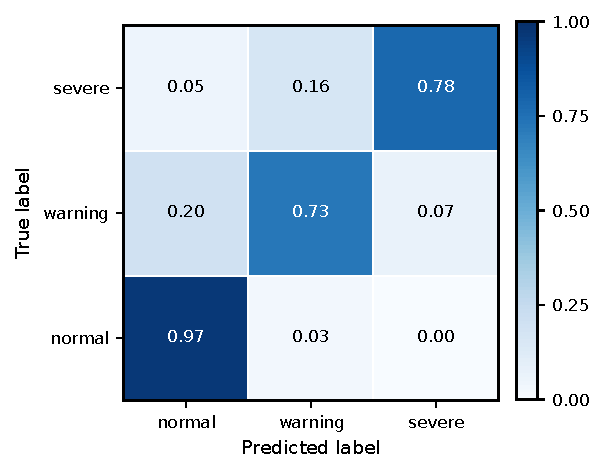
\includegraphics[width=\linewidth]{figures/confusion_matrix.pdf}
  \caption{Normalized confusion matrix, one registered \methodname{} run (TrafficCD, seed 17).}
\end{subfigure}\hfill
\begin{subfigure}{0.48\linewidth}
  \centering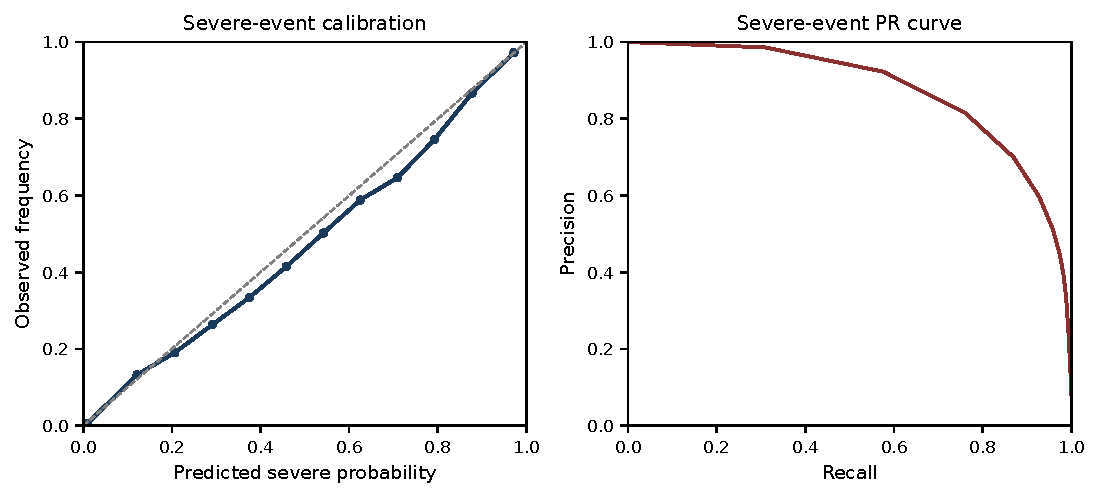
\includegraphics[width=\linewidth]{figures/calibration_pr.pdf}
  \caption{Severe-event calibration and PR curve, same run.}
\end{subfigure}
\caption{Qualitative diagnostics for one registered \methodname{} run. Source:
\texttt{outputs/studies/final\_study/main/TrafficCD/rugd/seed\_17/predictions.npz}; rendered by
\texttt{paper/figures/render\_figures.py}.}
\label{fig:qualitative}
\end{figure}

\Cref{fig:qualitative} (\Cref{sec:results-calib-eff}) gives the confusion matrix and severe-event
calibration/PR curves for one registered run (TrafficCD, seed 17). Errors concentrate between
\emph{adjacent} severity classes (normal$\to$warning: 2.95\% of true-normal examples; warning
$\to$severe and severe$\to$warning: 7.35\% and 16.47\% respectively) rather than the ordinally
distant normal$\leftrightarrow$severe confusion (0.31\% and 5.32\%), consistent with the label
space's ordinal structure even though the model is trained as an unordered 3-way classifier. We
did not curate additional qualitative failure-case examples (e.g., specific mispredicted road
segments or time windows) for this submission; the per-run \texttt{predictions.npz} files
(\texttt{time\_ids}, \texttt{node\_ids} arrays) support this directly as a follow-up.

\section{Derivations}
\label{app:derivations}

The Dirichlet-to-uniform KL divergence used in \Cref{eq:classification-loss}
(\texttt{src/traffic\_ml/losses.py::dirichlet\_kl\_to\_uniform}) is the standard closed form for
two Dirichlet distributions with concentration vectors $\boldsymbol\alpha,\boldsymbol\beta\in
\mathbb{R}_{>0}^K$:
\[
\mathrm{KL}[\mathrm{Dir}(\boldsymbol\alpha)\|\mathrm{Dir}(\boldsymbol\beta)]
= \log\frac{\Gamma(\sum_k\alpha_k)}{\Gamma(\sum_k\beta_k)} - \sum_k\log\frac{\Gamma(\alpha_k)}{\Gamma(\beta_k)}
+ \sum_k(\alpha_k-\beta_k)\big(\psi(\alpha_k)-\psi(\textstyle\sum_k\alpha_k)\big),
\]
with $\Gamma$ the gamma function and $\psi$ the digamma function; setting $\boldsymbol\beta=\mathbf 1$
recovers the uniform-Dirichlet target used throughout. \Cref{sec:analysis}'s analysis concerns
which entries of $\boldsymbol\alpha$ (equivalently $\tilde{\boldsymbol\alpha}$) are passed into this
formula, not the formula itself, which is implemented correctly against its own definition.

\section{Compute and Energy Reporting}
\label{app:compute}

Directly summing the \texttt{train\_seconds} and \texttt{inference\_seconds} columns across every
retained run gives 5{,}970s (main-suite training, 99 runs) + 5{,}693s (ablation training, 63 runs)
+ 14s + 7s (inference) $=$ 11{,}684s $\approx$ 3.25 GPU-hours for all main-suite and ablation
model-fit compute, plus 18{,}293s $\approx$ 5.08 GPU-hours for the 12 logged Optuna tuning searches
(RUGD/UIGNN/STAEformer-Inductive/OpenCity-Scratch only) --
\textbf{8.33 GPU-hours accounted for in total}, on one NVIDIA RTX 5080 (\texttt{environment.json}).
This explicitly excludes GRU/Graph-GRU's earlier, unretained tuning-pass compute (\Cref{sec:setup},
\Cref{sec:limitations}); we do not have a figure for that and do not estimate one. We did not
measure or estimate carbon emissions for this study.

\section{Reproducibility: Exact Commands}
\label{app:regenerate}

\begin{itemize}
  \item Full study from scratch: \texttt{python scripts/run\_full\_pipeline.py --study-id
        final\_reproduction --baseline-trials 30 --trials 20 --transformer-trials 8}
        (\texttt{--resume} to continue an interrupted run without repeating completed work).
  \item Verification before a long run: \texttt{python -m pytest -q} and
        \texttt{python scripts/verify\_modern\_models.py --batch-size 12 --backward}.
  \item Every number in every main-body and appendix table: \texttt{python
        paper/tables/generate\_tables.py}, reading only from
        \texttt{outputs/studies/final\_study/\{main,ablations\}/*.csv}.
  \item The headline table's bootstrap confidence intervals (\Cref{tab:headline}), using the same
        hierarchical city-then-seed bootstrap as every paired-comparison CI in this paper:
        \texttt{python paper/tables/regenerate\_headline\_ci.py}.
  \item Every figure's underlying data: \texttt{python
        paper/figures/regenerate\_figure\_data.py}.
  \item The Markdown results report this paper's numbers were cross-checked against:
        \texttt{python scripts/export\_results\_report.py} $\to$ \texttt{docs/FINAL\_RESULTS.md}.
\end{itemize}

\section{Material Relocated from the Prior Draft}
\label{app:relocated}

An earlier internal draft of this paper (never submitted; see the accompanying \texttt{
DRAFT\_TRIAGE.md} audit) contained the same core results reported here, independently re-verified
against the raw per-run CSVs during this revision (zero numeric discrepancies found). Two changes
from that draft are worth recording explicitly: (1) two subsections in that draft
("per-city ablations," "complete metric breakdown") consisted of a bare table with no interpretive
prose; the corresponding tables here (\Cref{tab:full-metrics}, and the per-city ablation numbers
folded into \Cref{app:complete-results}) are accompanied by explicit takeaways, per this paper's
own "never a table without a takeaway" standard; (2) that draft's architecture figure
(\Cref{fig:architecture}'s predecessor) was a raster illustration with decorative city-skyline
icons and no tensor-shape labels; \Cref{app:figure-redesign} documents the redesign.

\subsection{Figure redesign notes}
\label{app:figure-redesign}

The prior draft's Figure 1 used gradient-shaded blobs, decorative city-skyline icons, and
color-only encoding of block type, with no arrow-level tensor shapes and no notation tying it to
the Method section's equations. \Cref{fig:architecture} instead: (1) labels every block with the
paper's own symbols ($h_i$, $m_i$, $s_i$, $z_i$, $\alpha_i$) rather than icons; (2) annotates the
two main data-flow arrows with the fused/diffused representation symbols; (3) distinguishes
inference-path (solid) from training-only paths (dashed), a shape-redundant encoding (not
color-only) for colorblind accessibility, with the exact key given in the caption; (4) uses a
fixed, colorblind-safe palette defined locally in the figure source; (5) is pure vector TikZ with
no embedded raster content, compiling directly from \texttt{paper/figures/architecture.tex} via
\texttt{main.tex}.

This went through two internal revisions before the one in the main text. The first used
TikZ's \texttt{positioning} library (chained \texttt{right=X of Y} / \texttt{above right=X and Y
of Z} placements) rather than fixed coordinates; two independent chains that shared an anchor
node compounded their relative offsets unpredictably once rendered at full size, producing a
visible overlap between the local-evidential-head box and the diffusion block, and the legend
was built from a \texttt{matrix} of nested \texttt{\textbackslash tikz\{...\}} mini-pictures,
which is invalid outside an active \texttt{tikzpicture} context and caused a
"TeX capacity exceeded" runaway-expansion compile error. The second revision fixed both with
absolute coordinates and a legend built from plain nodes in the outer picture, but its natural
bounding box was roughly $26\times20$\,cm; scaling that down to the page width via
\texttt{\textbackslash resizebox} would have shrunk the font by the same factor as everything
else, past the point of legibility. The version in the main text compacts the coordinate grid to
roughly $19\times10.5$\,cm and moves the legend into the caption rather than drawing it in the
figure, which removes both the size problem and the class of nested-node risk that caused the
first revision's compile error, rather than only patching that one instance of it.


\bibliography{refs}

\end{document}
